% !TEX root = ../gamification-in-human-resource-management.tex
% !TeX program = xelatex
\chapter{کارهای پیشین}
در این فصل به تفصیل در مورد چند پیاده‌سازی ساده و جذاب از سناریوهای موفق مرتبط با مدیریت منابع انسانی صحبت خواهد شد. آنچه که در ادامه مطالعه می‌کنید، بر اساس بخش‌های مختلف فرایند مدیریت منابع انسانی جدا شده‌است.
\section{استخدام}
در مورد استخدام باید به دنبال طراحی بازی‌هایی باشیم که دارای تم‌های اصلی استخدام باشد، تم‌های اصلی استخدام به ترتیب در ذیل آمده‌اند:
\begin{itemize}
	\item طراحی برنامه‌ریزی شغلی
	\item شناخت مهارت‌های شغلی
	\item سنجش نوآوری
	\item توسعه زیرساخت‌های فناوری سازمان
	\item ویژگی‌های فردی
	\item شناخت سرمایه روانشناسی
	\item شناخت سرمایه اجتماعی
	\item قدرت تطبیق‌پذیری با اهداف شغلی
\end{itemize}
\subsection{بیلبوردهای گوگل}
در سال 2004 گوگل\LTRfootnote{Google} در بزرگراه 101 سان‌فرانسیسکو\LTRfootnote{San Francisco} که محل تردد کارمندان شرکت‌های معروفی مثل سیسکو\LTRfootnote{Cisco}، اپل\LTRfootnote{Apple}، ای‌بی\LTRfootnote{eBay} و غیره می‌باشد، یک بیلبورد رمزآلود با نوشته‌ای روی آن که صرفا می‌گفت \textit{اولین عدد اول ده‌رقمی که در دنباله نپر یافت می‌شود دات کام} نصب کرد (\xf{fig:google}) که افراد کنجکاو را وامی‌داشت تا معمای آن را حل کند که پس از حل معما و مراجعه به سایت مورد نظر\LTRfootnote{7182818284.com}، فرد با فرم تقاضای استخدام در گوگل مواجه می‌شود \cite{eprimesolve}.

\begin{figure}[!htb]
	\centering
	
\includegraphics[width=\textwidth]{Figures/eprime.jpg}
	\caption{بازی استخدامی گوگل که با یک بیلبورد پیاده‌سازی شد\cite{eprimepic}}
	\label{fig:google}
\end{figure}


گوگل بدون آنکه اسمی از خود در این بیلبورد برده باشد، با کمک این معما و طراحی یک بازی توانست در فرایند استخدام خود به خوبی روندی گزینشی را طی کند. با این کار گوگل می‌توانست افراد کنجکاو (بازیکنان جستجوگر) و برنامه‌نویسانی با حداقل‌های لازم علمی و فنی را پیدا کند و خصوصیاتی که لازم داشت را بدون نیاز به صرف زمان، به دست آورد.

\subsection{ارتش آمریکا}
ارتش آمریکا بازی ویدیویی \href{https://www.americasarmy.com/}{\lr{America's Army}} را  در سبک شوتر اول‌شخص در سال 2002 برای عموم منتشر کرد. روش انجام بازی به این صورت است که افراد در گروه‌هایی چندنفره قرار می‌گیرند که یکی از اعضا به عنوان رهبر گروه، چند نفر نقش پشتیبانی و چند نفر سرباز گروه تعیین می‌شوند. گروه‌های مختلف به مبارزه با یکدیگر می‌پردازند و با در نظر گرفتن تاکتیک‌ها و نقشه‌هایی سعی می‌کنند گروه‌های دیگر را از بین ببرند \cite{eventful}.

این بازی علاوه بر تبلیغ ارتش آمریکا باعث شده‌است که علاقه‌مندان به حضور در ارتش با کمک این بازی بتوانند شناخت و تجربه‌ای بهتر نسبت به فضای ارتش و محیط نظامی کسب کنند و از سمت دیگر خود ارتش بهتر می‌تواند توانایی‌های ذهنی، اجتماعی فرماندهی و مهارتی افراد متقاضی را متوجه شود \cite{army}.

ارتش آمریکا همچنین از طریق بستر اشتراک ویدیوی آنی توییچ\LTRfootnote{Twitch live stream} به رصد بازیکنان می‌پردازد و افرادی را که مهارت‌های مورد نظر ارتش را دارند، جذب می‌کند \cite{uhl, cbs}. ارتش آمریکا از بستر بازی‌های ویدیویی برای افزایش مهارت‌های نرم و قدرت مشارکت تیمی نیز بهره می‌برد \cite{cbs}.

\subsection{قهرمان پیتزا دومینو}
امیری و امین \cite{amiriamin} در مقاله خود این مثال را مطرح کرده‌اند. پیتزا دومینو بازی جذابی با نام قهرمان پیتزا دومینو\LTRfootnote{Domino's pizza hero} طراحی کرد که در طی این بازی افراد سعی می‌کنند پیتزای مورد علاقه خود را تهیه کند و عملیات آماده‌سازی تا پخت را انجام دهد. پیتزا دومینو متقاضیان استخدام در این فروشگاه را مجبور می‌کرد که در این بازی یک حساب کاربری بسازند و بازی کنند و از این طریق می‌توانست مهارت‌ها و سطح دانش متقاضی را بسنجد. از سمت دیگر این بازی برای پیتزا دومینو معروفیت و شهرت را نیز به همراه آورد و باعث شد که فروش این فروشگاه به میزان ماهانه یک میلیون دلار افزایش یابد.

بازی قهرمان پیتزا دومینو دو مزیت دیگر را نیز برای پیتزا دومینو به ارمغان آورد‌؛ یکی آنکه مشتریان با داستان این برند بهتر آشنا شدند و دیگر آنکه این بازی به عنوان محصولی جانبی برای پیتزا دومینو سودآوری خوبی هم داشت.
\begin{figure}[!htb]
	\centering
	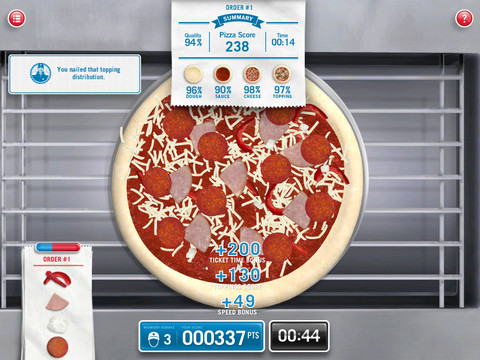
\includegraphics[width=\textwidth]{Figures/domino.png}
	\caption{نمایی از بازی قهرمان پیتزا دومینو \cite{domino}}
\end{figure}

\section{مدیریت عمل‌کرد و مشارکت}
قسمتی دیگر از فرایند مدیریت منابع انسانی بحث مدیریت عمل‌کرد و مشارکت است. سازمان‌های باید بتوانند نحوه کارکرد کارمندان را شناسایی کنند، آن را بهبود بخشند و در عمل‌کرد بین آن‌ها مشارکت ایجاد کنند \cite{review}.

برای ایجاد مشارکت بین کارمندان باید میزان رضایت شغلی افراد سنجیده شود. رضایت شغلی مبتنی بر ارزش‌ها و باورهای افراد شکل می‌گیرد و باید این موارد در فرایند ایجاد رضایت در افراد، در نظر گرفته شوند. زمانی که رضایت شغلی ایجاد می‌شود، کارمندان تمایل پیدا می‌کنند که به صورت خودجوش به تبلیغ سازمان بپردازند و مروجان سازمان باشند؛ بنابر این هنگام افزایش رضایت شغلی در کارمندان، علاوه بر بهبود عمل‌کرد کارمندان و ایجاد مشارکت، مزیت تبلیغ سازمان نیز رخ می‌دهد \cite{rezayat}.

طبق مطالعات چو \cite{actionable} گاهی مشارکت نتیجه مطلوبی ندارد و ایجاد رقابت بین کارمندان بهتر است. پیاده‌سازی روش‌های بازی‌وارسازی برای ایجاد مشارکت بین کارمندان و بهبود عمل‌کرد آن‌ها، مثل سایر قسمت‌ها نیازمند این است که جامعه بازیکنان سنجیده شود. در جامعه‌ای مثل ایران که فقر بازی به چشم می‌خورد و البته اکثر افراد از دسته قاتل‌ها هستند، این احتمال وجود دارد که بازی‌های مشارکتی و همکارانه مورد استقبال قرار نگیرند چون دید مناسب و مثبتی نسبت به این نوع بازی‌ها وجود ندارد \cite{atoz}. با استفاده از پرسش‌هایی که از افراد صورت می‌گیرد و تست‌های شخصیت به اضافه نگاه به فرهنگ سازمانی می‌توان دریافت که برای بهبود عمل‌کرد بین کارمندان بهتر است که رقابت ایجاد شود، مشارکت افزایش یابد یا ترکیبی از این دو در نظر گرفته‌شود \cite{reghmosh}.
\subsection{شبکه‌های اجتماعی کارمندان}
\label{sec:socialnetwork}
شبکه‌های اجتماعی سازمانی نوعی از شبکه‌های اجتماعی هستند که در آن افراد به تولید محتوای مرتبط با سازمان، دنبال‌کردن دیگر کارمندان و آشناشدن با دیگران (گسترش شبکه بین افراد) و اصلاح یا امتیازدهی به محتوای تولیدی دیگران می‌پردازند. بر اساس امتیازاتی که به محتواها داده می‌شود یک جدول برندگان تشکیل می‌شود و افراد رتبه‌بندی می‌شوند \cite{sharepoint}.
این شبکه‌های اجتماعی که عنصرهای مختلف بازی‌وارسازی را در خود به خوبی پیاده‌سازی می‌کنند علاوه بر ایجاد مشارکت به خاطر گسترش شبکه آشنایان کارمندان و همچنین ایجاد رقابت به دلیل مقایسه خود با دیگران، به سازمان‌ها کمک می‌کند که مدیریت دانش خوبی ایجاد کنند که این به بهبود عمل‌کرد آنان کمک می‌کند و البته تاریخچه‌ای نسبت به سازمان، اعضای سازمان و محتواهای تولیدشده مرتبط با اعضای فعلی و قدیمی سازمان برای کارمندان آینده جمع‌آوری می‌شود که در آموزش آن‌ها کمک‌کننده خواهد بود.

\begin{figure}[!htb]
	\centering
	\begin{minipage}[b]{0.49\textwidth}
		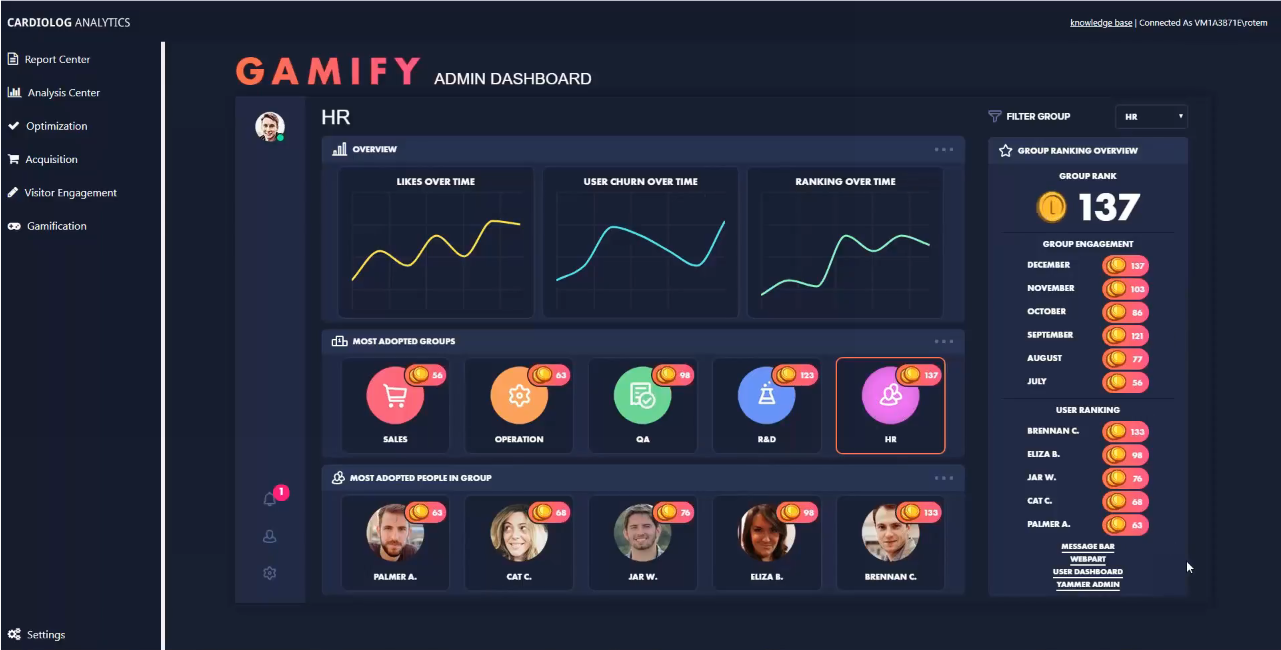
\includegraphics[width=\textwidth]{Figures/social1.png}
	\end{minipage}
	\begin{minipage}[b]{0.49\textwidth}
		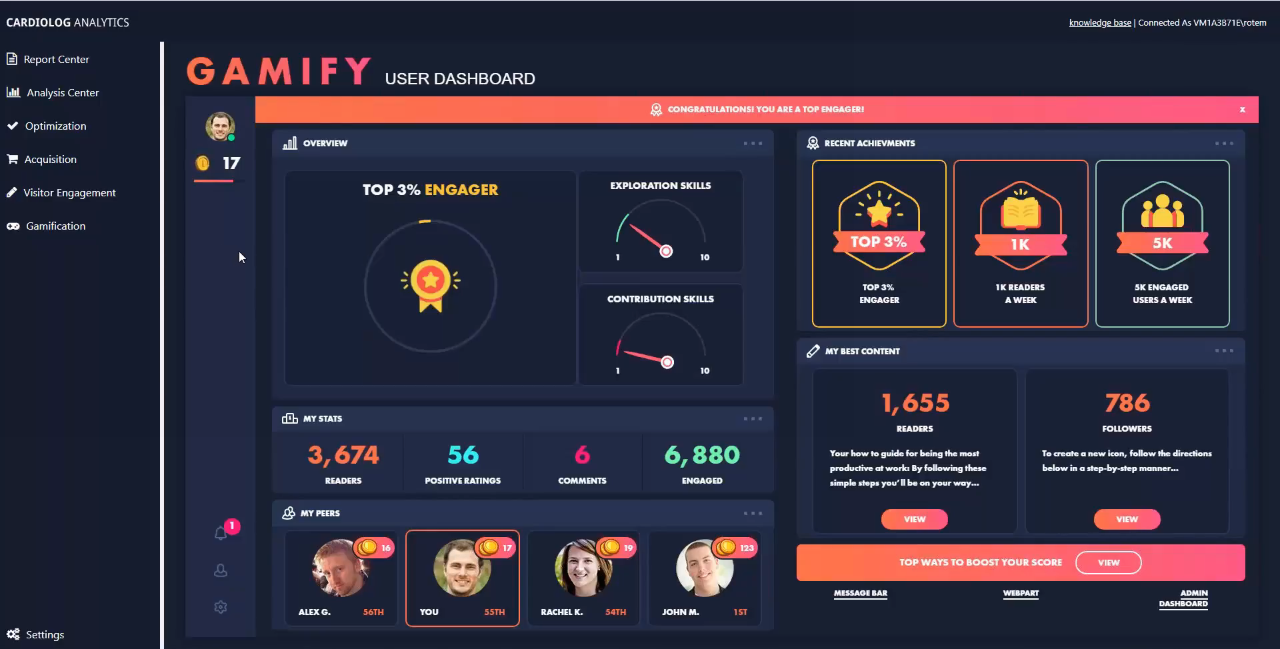
\includegraphics[width=\textwidth]{Figures/social2.png}
	\end{minipage}
	\caption{نمایی از شبکه اجتماعی مخصوص کارمندان یک سازمان\cite{sharepoint}}
\end{figure}

\subsection{بازی‌هایی برای بهبود جلسه‌های اداری}
در یک سخنرانی تد \cite{tedx} در مورد سازمانی صحبت شد که در تشکیل جلسه‌های سازمان، مشکلاتی مثل دیرکرد افراد، همهمه حین صحبت و طول‌کشیدن بیهوده زمان جلسه‌ها، وجود داشت و به همین خاطر سازمان سعی کرد با استفاده از سه ترفند به وضعیت جلسه‌ها نظم و کارآمدی را اضافه کند.
\begin{trick}[تیر هوایی]
هنگامی که جلسه شروع می‌شود، یک صدای بلند (می‌تواند شلیک هوایی واقعی باشد) در سازمان پخش می‌شود. این صدا به همه اعلام می‌کند که جلسه شروع شده‌است.
\end{trick}
\begin{trick}[ساعت جادویی]
یک ساعت خاص در جلسه وجود دارد که دقیقا روی ۱۵ دقیقه تنظیم شده‌است. زمانی که جلسه شروع شود، زمان‌سنج ساعت به جریان می‌افتد و سر ۱۵ دقیقه بعد، زنگ می‌زند. به این ترتیب جلسه طولانی نمی‌شود و در زمان مقرر پایان می‌یابد.
\end{trick}
\begin{trick}[پرندگان خشمگین\LTRfootnote{Angry birds}]
کسی که در حال صحبت است یک عروسک از بازی موبایلی پرندگان خشمگین در دست دارد؛ در حقیقت مجوز صحبت‌کردن برای هر کس این است که عروسک در دست او باشد. هنگامی که صحبت فرد پایان می‌یابد، عروسک را به طرف کسی که تمایل دارد صحبت کند، پرتاب می‌کند. به این شکل از همهمه در جلسات جلوگیری می‌شود و صحبت‌ها به نوبت انجام خواهند شد.
\end{trick}
\section{آموزش و استعداد}
بین آموزش و بهره‌وری ارتباط مستقیمی وجود دارد؛ به این شکل که هر مقدار در آموزش سرعت بالاتری داشته باشیم، در عمل‌کرد کارمندان شاهد بهبود بهره‌وری خواهیم بود. در این قسمت می‌توانیم از راهکارهای مرتبط با بازی‌وارسازی در آموزش استفاده کنیم که به چند مورد از آن‌ها در ادامه پرداخته می‌شود \cite{amiriamin}.
\subsection{اتاق فرار}\LTRfootnote{Escape room}
اتاق فرار یک بازی فیزیکی است که شامل یک اتاق و چند نفر زندانی است. زندانی‌ها باید با حل معماها و چالش‌های درون اتاق، راه فرار را پیدا کنند و خودشان را نجات دهند. این معماها و چالش‌ها در اکثر مواقع باید به صورت همکارانه حل شوند، گاهی به تحلیل علمی نیاز دارند و در بعضی از مواقع متکی به هوش خواهند بود \cite{atoz}.

استفاده از اتاق فرار برای آموزش می‌تواند به طراحان بازی کمک کند که توانایی علمی افراد را بسنجند و استعدادهای نهفته‌ی افراد را آشکار کنند. مثلا اگر فردی قدرت رهبری خوبی داشته باشد، در این بازی توانایی خود را به خوبی نشان می‌دهد.
\subsection{موشک تک‌دستی}
یک بازی ساده است که در آن افراد باید موشک‌های کاغذی درست کنند و یک قانون دارد! قانون بازی این است که هیچ‌کس حق ندارد از دو دست خود استفاده کند؛ یعنی، افراد باید تنها با یک دست موشک بسازند. بدیهی است که ساخت موشک صرفا با یک دست کاری سخت و حتی ناشدنی است، به همین خاطر، افراد نیاز پیدا می‌کنند که با مشارکت یکدیگر موشک را بسازند و در حقیقت دو دست از دو نفر برای ساخت موشک تشکیل داده شود \cite{tedx}.

زمانی که کارمندان شرکت در اتاق انتظار قرار دارند یا در حال سپری کردن وقتی آزاد هستند، به آن‌ها این بازی پیشنهاد داده می‌شود. این بازی به کارمندان آموزش می‌دهد که چگونه با یکدیگر تعامل کنند و درصد مشارکتشان بالاتر برود.
\section{مدیریت دانش}
مدیریت دانش هم به آموزش سریع‌تر کمک می‌کند و هم در عمل‌کرد افراد فعلی و آینده سازمان موثر است چراکه راه‌های پیموده‌شده برای حل مسائل را به آن‌ها نشان می‌دهد. مدیریت دانش به عنوان یکی از مهم‌ترین کارهای سازمان و البته در حین فرایند مدیریت منابع انسانی، نیازمند داشتن مشارکت خوبی بین کارمندان است. در سازمان دانش ارزشمند است \cite{kmanagement} و با وجود مشارکت بین اعضا می‌توان به بهبود دانش افراد و در نتیجه مدیریت دانش، دست پیدا کرد. بازی‌وارسازی با راهکارهایی مثل شبکه اجتماعی کارمندان (رجوع شود به زیربخش \ref{sec:socialnetwork}) می‌تواند در فرایند مدیریت دانش به سازمان کمک کند و انجام آن را تسریع کند \cite{amiriamin}.
\subsection{شرکت مشاوره‌ای \lr{Blue wolf}}
به نقل از \cite{modiran}، شرکت \lr{Blue wolf} با استفاده از روش‌های بازی‌وارسازی سعی کرد فرایند مدیریت دانش در سازمان را بهبود دهد؛ به همین خاطر در اولین اقدام \emph{بلندگو را به همه کارمندان داد} و از نشت اطلاعات سازمان جلوگیری نکرد. برای هر فرد در سایت این شرکت، یک صفحه شخصی یا یک صفحه گروهی (با مشارکت گروهی از کارمندان) وجود دارد که بر روی آن افراد به تولید محتوا می‌پردازند. از سمت سازمان برای تولید محتوا، امتیازها و نشان‌هایی در نظر گرفته می‌شود که به افراد اعطا می‌شود. این کارها باعث شد در تولید محتوا خلاقیت ایجاد شود و اعضا با مشارکت یکدیگر به فرایند مدیریت دانش کمک کنند. از سمت دیگر به خاطر انتقال دانش سازمان به بیرون از آن، به شهرت این شرکت افزوده شد و کارمندان آن اعتبار بیشتری پیدا کردند که این سبب شد مشاوران شرکت نسبت به گذشته ۵۷ درصد بیشتر فعالیت داشته باشند \cite{bluewolf}. در نهایت به خاطر افزایش دانش و اعتبار شرکت، دارایی‌های شرکت افزایش پیدا کرد.

\begin{figure}[!htb]
	\centering
	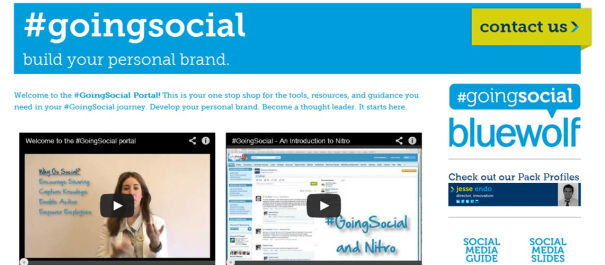
\includegraphics[width=\textwidth]{Figures/goingsocial.jpg}
	\caption{نمایی از سایت شرکت \lr{Blue wolf} \cite{goingsocial}}
\end{figure}

\section{فرهنگ سازمانی}
در بحث فرهنگ سازمانی مجددا دانش، مشارکت و مدیریت این موارد مطرح می‌شود اما فرهنگ باید در افراد نهادینه شود. هر میزان که نهادینه‌سازی فرهنگ در افراد سریع‌تر باشد، عمل‌کرد افراد و توانایی مشارکت بین آن‌ها افزایش پیدا می‌کند. لازمه انتقال فرهنگ، انتقال آگاهی است. این کار با استفاده از یک بازی سازمانی مبتنی بر بازی جومانجی\LTRfootnote{Jumanji} قابل انجام است \cite{amiriamin}.
\subsection{مدل بازی جومانجی}
بازی جومانجی یک بازی رومیزی\LTRfootnote{Boardgame} است که در آن هر شخصیت دارای یک قدرت ویژه است  که با این قدرت‌ها باید با خود بازی مبارزه کنند تا همه پیروز از بازی خارج شوند. این مدل در سایت مسترگیمیفیکیشن \cite{jumanji} مطرح شده‌است.

یک بازی سازمانی بر اساس این بازی می‌توان ساخت که در آن بازیکنان افراد تازه‌وارد به سازمان هستند، هر کدام از آن‌ها یک قدرت خاص دارند و هدف یافتن مدبرعامل است. در اولین روز کاری، قبل از شروع بازی تمام امکاناتی که به کارمندان تازه‌وارد در تقلب‌کردن کمک می‌کند (مثل تلفن همراه یا لپتاپ) از آن‌ها گرفته می‌شود. قدرت‌های خاص بازیکنان می‌تواند توانایی مصاحبه با بخش بازاریابی، استفاده محدود از تلفن همراه یا موارد دیگر باشد که با مشارکت بین افراد و جمع‌شدن قدرت‌ها افراد می‌توانند به هدف بازی یعنی یافتن مدیر عامل برسند.

هنگامی که مدیرعامل پیدا می‌شود، اعضای تازه‌وارد با مدیرعامل جشن می‌گیرند و به یک مهمانی دعوت می‌شوند. 
این بازی باعث می‌شود افراد تازه‌وارد به سرعت با فرهنگ سازمانی و محیط شرکت آشنا شوند، با دیگر افراد سازمان آشنا شوند و شبکه آن‌ها گسترش پیدا کند و البته نسبت به یکدیگر درک بیشتری پیدا می‌کنند. به علاوه این موارد باعث می‌شود که افراد خاطره خوبی از اولین روز کاری خود در سازمان داشته باشند و حتی در صورتی که سازمان را ترک کنند، این خاطره از ذهن آن‌ها پاک نمی‌شود.
